% =====================================================================
%  Aureus ERP - Accounting Pipeline Verification & Defect Report
%
%  Compile with pdflatex (run twice so the ToC resolves):
%      pdflatex accounting-verification-report.tex
%      pdflatex accounting-verification-report.tex
%
%  Requires a standard TeX distribution (TeX Live / MiKTeX) with tikz,
%  booktabs, xcolor, geometry, fontspec-free (uses default fonts so it
%  compiles with pdflatex out of the box).
% =====================================================================
\documentclass[11pt,a4paper]{article}

\usepackage[T1]{fontenc}
\usepackage[utf8]{inputenc}
\usepackage[margin=2.4cm]{geometry}
\usepackage{booktabs}
\usepackage{tabularx}
\usepackage{xcolor}
\usepackage{tikz}
\usepackage{graphicx}
\usepackage{enumitem}
\usepackage{titlesec}
\usepackage[hidelinks]{hyperref}
\usepackage{caption}

\usetikzlibrary{shapes.geometric, arrows.meta, positioning, calc, fit, backgrounds}

% ---------------------------------------------------------------- colours
\definecolor{ink}{HTML}{15191E}
\definecolor{inksoft}{HTML}{39424C}
\definecolor{muted}{HTML}{5F6A76}
\definecolor{rule}{HTML}{D8DEE3}
\definecolor{surface}{HTML}{F4F6F7}
\definecolor{accent}{HTML}{0F5C5C}
\definecolor{critical}{HTML}{9D2B2B}
\definecolor{high}{HTML}{9A5A12}

% ---------------------------------------------------------------- styling
\titleformat{\section}{\Large\bfseries\color{ink}}{\thesection}{0.7em}{}
\titleformat{\subsection}{\large\bfseries\color{ink}}{\thesubsection}{0.7em}{}
\titlespacing*{\section}{0pt}{20pt}{8pt}

\captionsetup{font=small, labelfont={bf,color=accent}, width=0.92\textwidth}
\setlist{itemsep=2pt, topsep=4pt, parsep=0pt}

\newcommand{\sev}[2]{\textcolor{#1}{\small\textsf{\textbf{#2}}}}
\newcommand{\acct}[1]{\texttt{\small #1}}

% ------------------------------------------------------------ tikz styles
\tikzset{
  box/.style      = {draw=inksoft, line width=0.7pt, rectangle, rounded corners=1pt,
                     align=center, inner sep=6pt, minimum height=11mm, font=\small},
  boxsoft/.style  = {box, draw=rule, fill=surface, text=inksoft},
  boxhl/.style    = {box, draw=accent, line width=1.1pt, text=accent, font=\small\bfseries},
  boxbad/.style   = {box, draw=critical, line width=1.0pt, text=critical},
  flow/.style     = {-{Stealth[length=2mm]}, draw=inksoft, line width=0.7pt},
  flowdash/.style = {flow, dashed},
  note/.style     = {font=\scriptsize\itshape, text=muted, align=center},
  entry/.style    = {font=\scriptsize\ttfamily, text=inksoft, align=center},
}

% =====================================================================
\begin{document}

\begin{titlepage}
\vspace*{3cm}
{\footnotesize\textsf{\textcolor{accent}{AUREUS ERP \quad$\cdot$\quad ACCOUNTING MODULE}}}\\[1.1em]
{\Huge\bfseries Accounting Pipeline\\[0.25em] Verification \& Defect Report}\\[1.6em]
{\large\color{inksoft}
Manual end-to-end testing of the accounting module against a real trucking-company
scenario, the defects that testing exposed, and the fixes and regression tests now
covering them.}\\[2.5em]
\begin{tabular}{@{}ll@{}}
\textsf{\small\textbf{Test entity}} & Truck It In (Private) Limited\\[2pt]
\textsf{\small\textbf{Period}}      & September 2026\\[2pt]
\textsf{\small\textbf{Status}}      & All identified defects resolved\\
\end{tabular}
\vfill
{\footnotesize\color{muted}
Laravel / Filament / MySQL. Verification performed against the development database through
the application interface, with all ledger effects confirmed by direct database inspection.
Test entity, customer and transaction data are fictional.}
\end{titlepage}

\tableofcontents
\newpage

% =====================================================================
\section{Summary}

The accounting module was tested by working a complete real-world bookkeeping cycle through
the application interface --- company setup, chart of accounts import, capital injection, asset
purchase, customer invoicing, payment collection and bank reconciliation --- rather than by
reading code or running the existing test suite in isolation.

That approach mattered. \textbf{Two of the defects found were capable of silently corrupting the
general ledger}, and neither was caught by the existing 79-test suite, because the test fixtures
pre-set the very fields that were broken in production use. Both are now covered by tests that
were confirmed to fail against the original code before the fix was applied.

\vspace{6pt}
\noindent\fcolorbox{rule}{surface}{%
\begin{minipage}{0.96\textwidth}
\vspace{4pt}
\textbf{Headline finding.} Invoices could be saved with their line items silently deleted, and
separately, unpaid invoices reported themselves as fully paid. Either defect alone would produce
materially wrong financial statements without any error being shown to the user.
\vspace{4pt}
\end{minipage}}

\vspace{14pt}
\begin{center}
\begin{tabular}{@{}cccc@{}}
\toprule
\textbf{7} & \textbf{9} & \textbf{8} & \textbf{15}\\
\footnotesize\textsf{workflows tested} & \footnotesize\textsf{defects fixed} &
\footnotesize\textsf{regression tests added} & \footnotesize\textsf{source files changed}\\
\bottomrule
\end{tabular}
\end{center}

% =====================================================================
\section{Method}

A fictional but realistic entity --- a Pakistani trucking company --- was set up from scratch and
its transactions entered through the normal user interface. After each step the resulting journal
entries were verified directly against the database, rather than trusting the on-screen totals.
Where the system's behaviour diverged from what double-entry accounting requires, work stopped and
the responsible code was traced before anything was changed.

\subsection{Workflows exercised}

\begin{enumerate}[leftmargin=*]
  \item \textbf{Company and currency setup.} Entity created with PKR as functional currency.
  \item \textbf{Chart of accounts import.} 17 accounts imported via CSV covering bank, receivables,
        fixed assets, payables, equity, revenue and expenses.
  \item \textbf{Capital injection.} PKR 5,000,000 of share capital.\\
        \acct{Dr 1010 Bank 5,000,000 \quad Cr 3010 Share Capital 5,000,000}
  \item \textbf{Fixed asset purchase.} Delivery vehicle for PKR 1,800,000.\\
        \acct{Dr 1510 Delivery Vehicles 1,800,000 \quad Cr 1010 Bank 1,800,000}
  \item \textbf{Customer invoicing.} Freight service invoiced and posted.\\
        \acct{Dr 1020 Trade Debts \quad Cr 4010 Freight Revenue}
  \item \textbf{Payment collection.} Payment registered through a bank journal.\\
        \acct{Dr 1030 Outstanding Receipts \quad Cr 1020 Trade Debts}
  \item \textbf{Bank reconciliation.} Statement imported, auto-matched to the open invoice,
        approved and posted; an unrecorded bank charge classified manually.\\
        \acct{Dr 1010 Bank \quad Cr 1020 Trade Debts} \quad$|$\quad
        \acct{Dr 5050 Bank Charges \quad Cr 1010 Bank}
\end{enumerate}

The reconciliation closed cleanly: the bank ledger finished at \textbf{PKR 3,846,500}, exactly
matching the imported statement's closing balance, with every statement line accounted for and the
statement marked complete by the system.

% =====================================================================
\newpage
\section{System flows}

Each complete flow in the accounting module, as verified during testing. These describe how the
system behaves after the fixes in this report.

% ---------------------------------------------------------------- fig 1
\subsection{The accounting cycle}

\begin{figure}[h!]
\centering
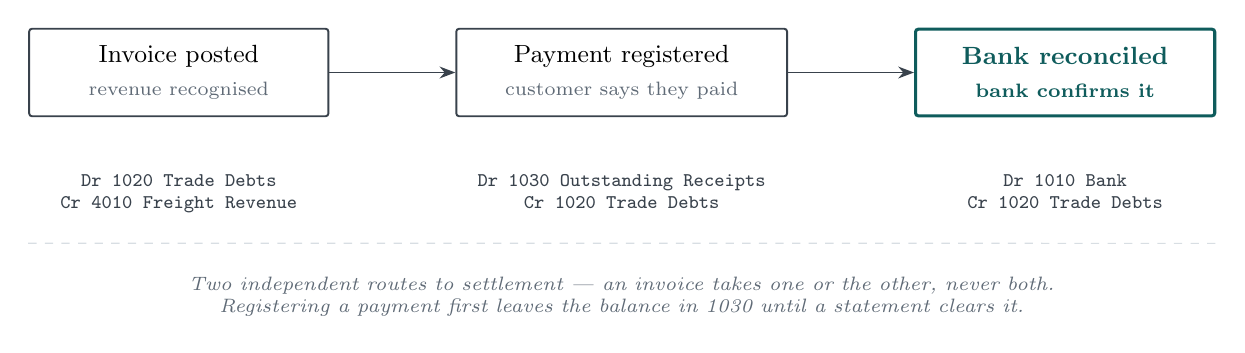
\begin{tikzpicture}[node distance=8mm]
  \node[box, minimum width=38mm] (inv) {Invoice posted\\[1pt]{\scriptsize\color{muted}revenue recognised}};
  \node[box, minimum width=42mm, right=16mm of inv] (pay) {Payment registered\\[1pt]{\scriptsize\color{muted}customer says they paid}};
  \node[boxhl, minimum width=38mm, right=16mm of pay] (bank) {Bank reconciled\\[1pt]{\scriptsize\color{accent}bank confirms it}};

  \draw[flow] (inv) -- (pay);
  \draw[flow] (pay) -- (bank);

  \node[entry, below=6mm of inv]  {Dr 1020 Trade Debts\\ Cr 4010 Freight Revenue};
  \node[entry, below=6mm of pay]  {Dr 1030 Outstanding Receipts\\ Cr 1020 Trade Debts};
  \node[entry, below=6mm of bank] {Dr 1010 Bank\\ Cr 1020 Trade Debts};

  \draw[dashed, draw=rule] ($(inv.south west)+(0,-16mm)$) -- ($(bank.south east)+(0,-16mm)$);
  \node[note, below=19mm of pay, text width=110mm]
    {Two independent routes to settlement --- an invoice takes one or the other, never both.\\
     Registering a payment first leaves the balance in 1030 until a statement clears it.};
\end{tikzpicture}
\caption{The accounting cycle. The middle stage is optional: a customer payment either goes
through the clearing account (recorded before the bank confirms it) or is settled directly from
the bank statement. Using both on one invoice double-counts the receivable.}
\end{figure}

% ---------------------------------------------------------------- fig 2
\subsection{Chart of accounts import}

\begin{figure}[h!]
\centering
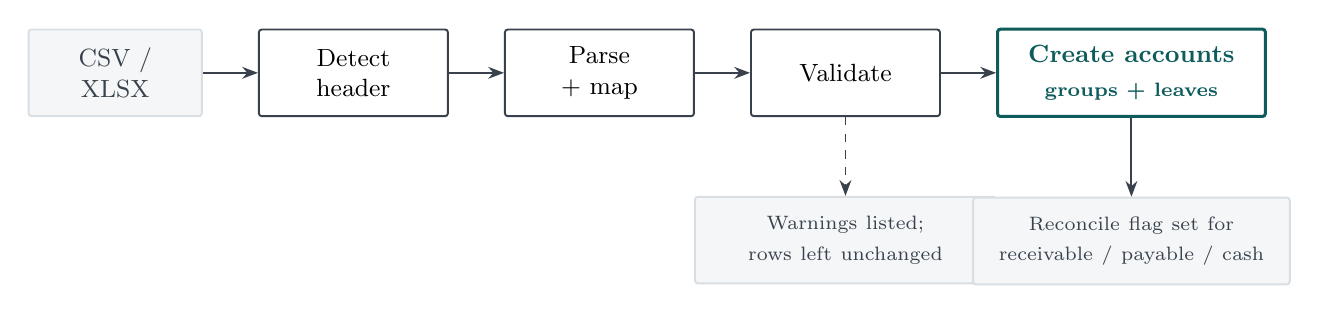
\begin{tikzpicture}
  \node[boxsoft, minimum width=22mm] (file) {CSV /\\XLSX};
  \node[box, minimum width=24mm, right=7mm of file] (hdr) {Detect\\header};
  \node[box, minimum width=24mm, right=7mm of hdr] (parse) {Parse\\+ map};
  \node[box, minimum width=24mm, right=7mm of parse] (val) {Validate};
  \node[boxhl, minimum width=34mm, right=7mm of val] (create) {Create accounts\\[1pt]{\scriptsize groups + leaves}};

  \draw[flow] (file) -- (hdr);
  \draw[flow] (hdr) -- (parse);
  \draw[flow] (parse) -- (val);
  \draw[flow] (val) -- (create);

  \node[boxsoft, below=10mm of val, text width=34mm] (warn) {\scriptsize Warnings listed;\\ rows left unchanged};
  \draw[flowdash] (val) -- (warn);

  \node[boxsoft, below=10mm of create, text width=36mm] (flag)
    {\scriptsize Reconcile flag set for\\ receivable / payable / cash};
  \draw[flow] (create) -- (flag);
\end{tikzpicture}
\caption{Chart of accounts import. Validation reports problems without altering the source rows.
The final step --- setting the reconcile flag by account type --- was missing before this report's
fix, which is what made unpaid invoices report as paid.}
\end{figure}

% ---------------------------------------------------------------- fig 3
\subsection{Invoice creation and posting}

\begin{figure}[h!]
\centering
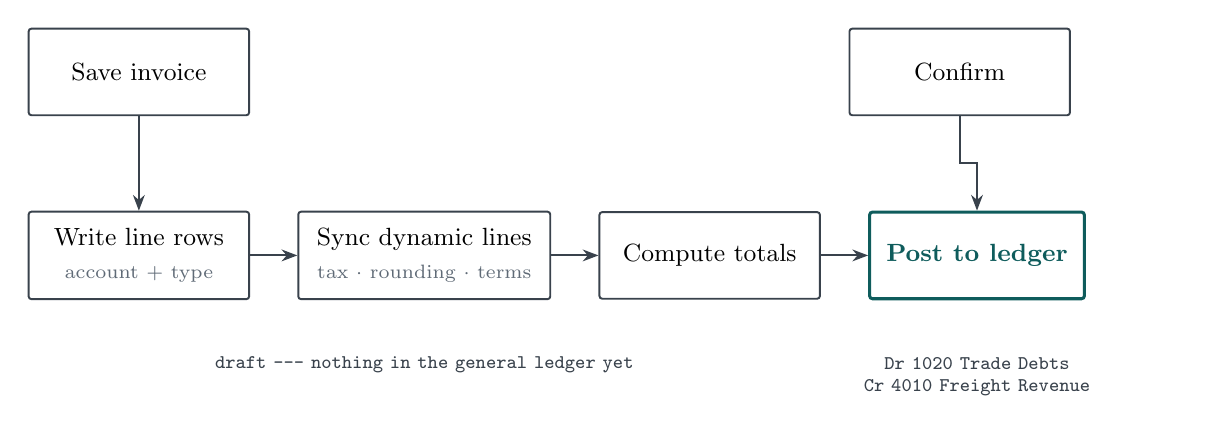
\begin{tikzpicture}
  \node[box, minimum width=28mm] (save) {Save invoice};
  \node[box, minimum width=28mm, right=76mm of save] (confirm) {Confirm};

  \node[box, minimum width=28mm, below=12mm of save] (write) {Write line rows\\[1pt]{\scriptsize\color{muted}account + type}};
  \node[box, minimum width=32mm, right=6mm of write] (sync) {Sync dynamic lines\\[1pt]{\scriptsize\color{muted}tax $\cdot$ rounding $\cdot$ terms}};
  \node[box, minimum width=28mm, right=6mm of sync] (tot) {Compute totals};
  \node[boxhl, minimum width=26mm, right=6mm of tot] (post) {Post to ledger};

  \draw[flow] (save) -- (write);
  \draw[flow] (write) -- (sync);
  \draw[flow] (sync) -- (tot);
  \draw[flow] (tot) -- (post);
  \draw[flow] (confirm) |- ($(post.north)+(0,6mm)$) -- (post);

  \node[entry, below=6mm of sync, text width=60mm] {draft --- nothing in the general ledger yet};
  \node[entry, below=6mm of post, text width=52mm] {Dr 1020 Trade Debts\\ Cr 4010 Freight Revenue};
\end{tikzpicture}
\caption{Invoice creation and posting. Everything left of \emph{Post to ledger} is reversible draft
state. Only confirming writes the double entry, which is why a draft invoice never appears in the
trial balance.}
\end{figure}

% ---------------------------------------------------------------- fig 4
\newpage
\subsection{Line account resolution --- the critical defect}

\begin{figure}[h!]
\centering
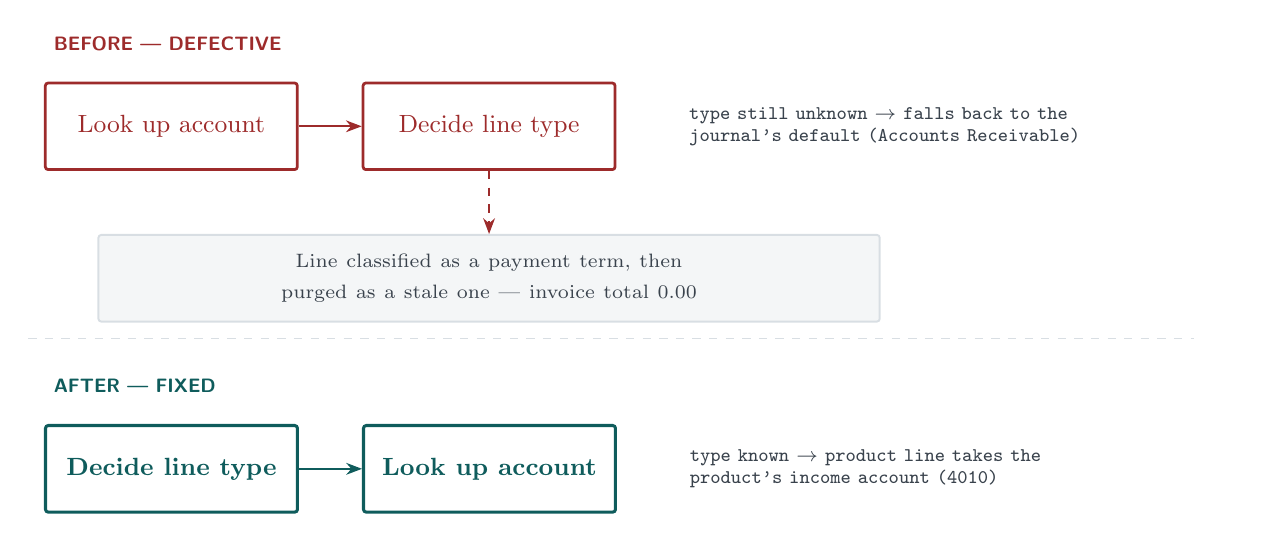
\begin{tikzpicture}
  % before
  \node[font=\scriptsize\sffamily\bfseries, text=critical, anchor=west] at (0,1.05) {BEFORE --- DEFECTIVE};
  \node[boxbad, minimum width=32mm, anchor=west] (b1) at (0,0) {Look up account};
  \node[boxbad, minimum width=32mm, right=8mm of b1] (b2) {Decide line type};
  \draw[flow, draw=critical] (b1) -- (b2);
  \node[entry, anchor=west, text width=68mm, align=left] at ($(b2.east)+(8mm,0)$)
    {type still unknown $\rightarrow$ falls back to the\\ journal's default (Accounts Receivable)};

  \node[boxsoft, below=8mm of b2, text width=95mm] (bad)
    {\scriptsize Line classified as a payment term, then purged as a stale one --- invoice total 0.00};
  \draw[flowdash, draw=critical] (b2) -- (bad);

  \draw[dashed, draw=rule] (-0.2,-2.7) -- (14.6,-2.7);

  % after
  \node[font=\scriptsize\sffamily\bfseries, text=accent, anchor=west] at (0,-3.3) {AFTER --- FIXED};
  \node[boxhl, minimum width=32mm, anchor=west] (a1) at (0,-4.35) {Decide line type};
  \node[boxhl, minimum width=32mm, right=8mm of a1] (a2) {Look up account};
  \draw[flow, draw=accent] (a1) -- (a2);
  \node[entry, anchor=west, text width=68mm, align=left] at ($(a2.east)+(8mm,0)$)
    {type known $\rightarrow$ product line takes the\\ product's income account (4010)};
\end{tikzpicture}
\caption{The one edge that changed. Two computations in the line's save sequence ran in the wrong
order. The account lookup branches on the line type, so running it first meant the type was never
available --- the line took the sales journal's receivable account and was then deleted as a
duplicate payment-term line.}
\end{figure}

% ---------------------------------------------------------------- fig 5
\subsection{Payment registration}

\begin{figure}[h!]
\centering
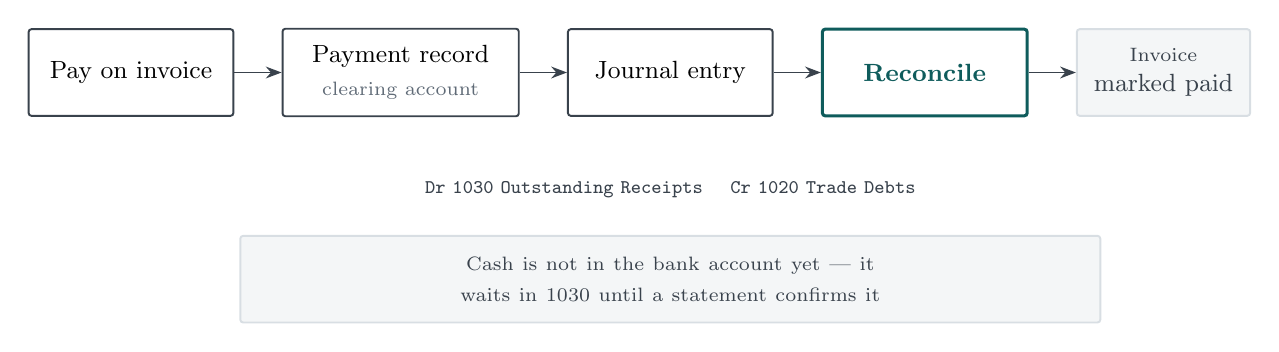
\begin{tikzpicture}
  \node[box, minimum width=26mm] (p1) {Pay on invoice};
  \node[box, minimum width=30mm, right=6mm of p1] (p2) {Payment record\\[1pt]{\scriptsize\color{muted}clearing account}};
  \node[box, minimum width=26mm, right=6mm of p2] (p3) {Journal entry};
  \node[boxhl, minimum width=26mm, right=6mm of p3] (p4) {Reconcile};
  \node[boxsoft, minimum width=22mm, right=6mm of p4] (p5) {\scriptsize Invoice\\ marked paid};

  \draw[flow] (p1) -- (p2);
  \draw[flow] (p2) -- (p3);
  \draw[flow] (p3) -- (p4);
  \draw[flow] (p4) -- (p5);

  \node[entry, below=7mm of p3, text width=80mm]
    {Dr 1030 Outstanding Receipts \quad Cr 1020 Trade Debts};
  \node[boxsoft, below=15mm of p3, text width=105mm]
    {\scriptsize Cash is not in the bank account yet --- it waits in 1030 until a statement confirms it};
\end{tikzpicture}
\caption{Payment registration. Recording a payment settles the receivable but deliberately does not
touch the bank account. The balance sits in a clearing account, so the ledger never claims money the
bank has not yet confirmed.}
\end{figure}

% ---------------------------------------------------------------- fig 6
\newpage
\subsection{Bank statement import and reconciliation}

\begin{figure}[h!]
\centering
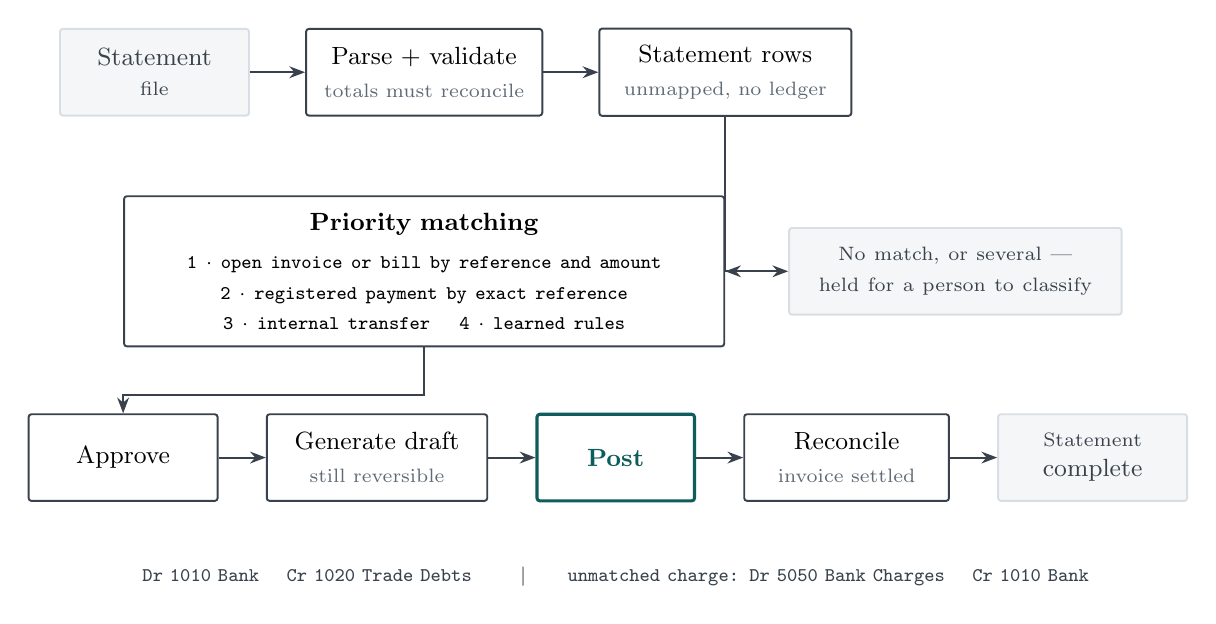
\begin{tikzpicture}
  \node[boxsoft, minimum width=24mm] (s1) {Statement\\{\scriptsize file}};
  \node[box, minimum width=30mm, right=7mm of s1] (s2) {Parse + validate\\[1pt]{\scriptsize\color{muted}totals must reconcile}};
  \node[box, minimum width=32mm, right=7mm of s2] (s3) {Statement rows\\[1pt]{\scriptsize\color{muted}unmapped, no ledger}};
  \draw[flow] (s1) -- (s2);
  \draw[flow] (s2) -- (s3);

  \node[box, below=10mm of s2, text width=72mm, align=center] (match)
    {\textbf{Priority matching}\\[3pt]
     {\scriptsize\ttfamily 1 $\cdot$ open invoice or bill by reference and amount}\\
     {\scriptsize\ttfamily 2 $\cdot$ registered payment by exact reference}\\
     {\scriptsize\ttfamily 3 $\cdot$ internal transfer \quad 4 $\cdot$ learned rules}};
  \draw[flow] (s3) |- (match);

  \node[boxsoft, right=8mm of match, text width=38mm] (hold)
    {\scriptsize No match, or several --- held for a person to classify};
  \draw[flow] (match) -- (hold);

  \node[box, minimum width=24mm] (ap) at ($(match.south west)+(0,-14mm)$) {Approve};
  \node[box, minimum width=28mm, right=6mm of ap] (dr) {Generate draft\\[1pt]{\scriptsize\color{muted}still reversible}};
  \node[boxhl, minimum width=20mm, right=6mm of dr] (po) {Post};
  \node[box, minimum width=26mm, right=6mm of po] (rec) {Reconcile\\[1pt]{\scriptsize\color{muted}invoice settled}};
  \node[boxsoft, minimum width=24mm, right=6mm of rec] (done) {\scriptsize Statement\\ complete};

  \draw[flow] (match.south) -- ++(0,-6mm) -| (ap.north);
  \draw[flow] (ap) -- (dr);
  \draw[flow] (dr) -- (po);
  \draw[flow] (po) -- (rec);
  \draw[flow] (rec) -- (done);

  \node[entry, below=7mm of po, text width=130mm]
    {Dr 1010 Bank \quad Cr 1020 Trade Debts \qquad$|$\qquad
     unmatched charge: Dr 5050 Bank Charges \quad Cr 1010 Bank};
\end{tikzpicture}
\caption{Bank statement import and reconciliation. Importing writes no ledger entries at all ---
only rows awaiting review. Matching produces a \emph{suggestion}; a person approves it, and posting
is a separate deliberate step. A bad import therefore cannot reach the books.}
\end{figure}

% =====================================================================
\newpage
\section{Defects found and fixed}

\subsection[Invoice line items silently deleted on save]{Invoice line items silently deleted on save \hfill \sev{critical}{CRITICAL}}

\begin{description}[leftmargin=!, labelwidth=2.4cm, font=\small\sffamily\bfseries\color{muted}]
  \item[Symptom] An invoice saved with a correct line item and total would open showing no lines and
    a total of 0.00. No error was displayed. Database inspection confirmed zero line rows existed.
  \item[Root cause] In the move line's save hook, the account lookup ran \emph{before} the line's
    display type was determined, but the lookup branches on that display type. For a new line it fell
    through to a default branch and assigned the journal's default account --- Accounts Receivable on a
    sales journal. The line was then reclassified as a payment-term line and subsequently purged as a
    stale one.
  \item[Fix] Reordered the two computations so display type is resolved first, and added a null guard
    now that the account is legitimately unset at that point.
  \item[Verification] Five regression tests that create lines exactly as the interface does. Confirmed
    failing against the original code (\acct{0 is identical to 1} --- the line count collapsing),
    passing after.
  \item[Scope] Affected customer invoices, vendor bills, credit notes and refunds --- all four screens
    rely on the same model logic. Fixing it at the model level resolved all of them.
\end{description}

\subsection[Unpaid invoices reported as fully paid]{Unpaid invoices reported as fully paid \hfill \sev{critical}{CRITICAL}}

\begin{description}[leftmargin=!, labelwidth=2.4cm, font=\small\sffamily\bfseries\color{muted}]
  \item[Symptom] A posted invoice for PKR 500,000 showed payment status \emph{Paid} with zero amount
    due, despite no payment existing anywhere in the system.
  \item[Root cause] Outstanding-balance calculation is skipped entirely for accounts not flagged as
    reconcilable, defaulting the residual to zero --- and zero residual is read as ``paid''. Neither the
    chart-of-accounts importer nor the manual account-creation service set that flag for receivable or
    payable accounts.
  \item[Fix] Added a single source of truth on the account-type enum defining which types must be
    reconcilable, and applied it in both creation paths. Backfilled 20 existing accounts and recomputed
    all affected invoices.
  \item[Verification] Two regression tests, confirmed failing before the fix. The affected invoice now
    correctly reports 500,000 outstanding; a genuinely paid invoice correctly remained paid.
  \item[Note] This defect was masked until the company-isolation fix below was applied --- invoices had
    been posting to another company's receivable account, which happened to carry the flag.
\end{description}

\subsection[Cross-company ledger contamination]{Cross-company ledger contamination \hfill \sev{high}{HIGH}}

\begin{description}[leftmargin=!, labelwidth=2.4cm, font=\small\sffamily\bfseries\color{muted}]
  \item[Symptom] Transactions belonging to the test entity posted to general ledger accounts owned by
    a different company in the same installation.
  \item[Root cause] Two independent paths. The customer/vendor form's receivable and payable account
    pickers listed every account in the system and defaulted to the lowest-numbered match, regardless of
    company. Separately, the outstanding-payments account is drawn from a single global setting with no
    per-company dimension, so every company resolved to whichever account was configured first.
  \item[Fix] Scoped the account pickers to the active company, and made outstanding-account resolution
    prefer an account belonging to the payment's own company before falling back to the global default.
  \item[Residual risk] The underlying settings architecture is still global rather than per-company.
    This is noted as an open item; the fix prevents the observed contamination but does not restructure
    that design.
\end{description}

\subsection[Company data visible across companies in list views]{Company data visible across companies in list views \hfill \sev{high}{HIGH}}

\begin{description}[leftmargin=!, labelwidth=2.4cm, font=\small\sffamily\bfseries\color{muted}]
  \item[Symptom] The invoice list displayed another company's invoices alongside the test entity's own
    records.
  \item[Root cause] Invoice, bill, payment, journal entry and journal item list queries applied no
    company filter.
  \item[Fix] Added company scoping to the base resources, covering both application panels from one
    change. On the journal entry screen the existing permission-scoping trait was aliased rather than
    overridden, so permission filtering still applies.
  \item[Verification] Confirmed programmatically as the admin user: records visible from other companies
    dropped to zero across all six lists, with the invoice list narrowing from 21 records to the entity's
    own 2.
\end{description}

\subsection[Bank matching would double-settle a receivable]{Bank matching would double-settle a receivable \hfill \sev{high}{HIGH}}

\begin{description}[leftmargin=!, labelwidth=2.4cm, font=\small\sffamily\bfseries\color{muted}]
  \item[Symptom] When a bank statement line matches a payment that was already registered in the
    system, the generated entry would credit the receivable a second time, driving it negative.
  \item[Root cause] The matcher preferred the payment's destination account (the receivable) over its
    outstanding clearing account. Registering a payment has already cleared the receivable, so the bank
    line must clear the clearing account instead.
  \item[Fix] Inverted the preference, retaining the destination account as a fallback for payments that
    never generated a clearing entry.
  \item[Verification] New regression test covering this path, which had no prior coverage. Confirmed
    failing before the fix.
\end{description}

\subsection{Lower-severity items, also resolved}

\begin{center}
\small
\begin{tabularx}{\textwidth}{@{}l X l@{}}
\toprule
\textbf{Item} & \textbf{Issue and resolution} & \textbf{Severity}\\
\midrule
Partner account query & Filtered on a database column that does not exist; would have thrown a SQL
  error whenever that path executed. Rewritten to filter on account type. & Latent crash\\
\addlinespace
Line classification & Receipt-type documents were excluded from tax and payment-term inference,
  inconsistent with sibling methods. Aligned with the rest of the module. & Latent\\
\addlinespace
Bank journal entries & Posted entries remained named ``Draft \ldots'', misleading in ledger reports.
  Renamed on posting. & Cosmetic\\
\addlinespace
Duplicate general journals & Two identically named journals; the entity's two manual entries had
  unknowingly used different ones. Disambiguated and missing currency set. & Data\\
\addlinespace
Bank journal code & No code set, producing malformed entry numbering. Code assigned. & Data\\
\bottomrule
\end{tabularx}
\end{center}

\vspace{6pt}
One further item was investigated and deliberately \textbf{not} changed: a currency computation reads
a display type that is set later in the same sequence. The branch is unreachable in the current
codebase, and altering working code for a theoretical case carries more risk than it removes. It is
documented rather than modified.

% =====================================================================
\section{Test coverage}

The existing suite passed both before and after these defects existed, which is itself a finding: the
test helper pre-set the two fields that were broken, so the failing code path was never exercised. The
new tests deliberately construct records the way the application does at runtime.

\begin{center}
\small
\begin{tabularx}{\textwidth}{@{}l X r l@{}}
\toprule
\textbf{Suite} & \textbf{Covers} & \textbf{Tests} & \textbf{Result}\\
\midrule
\acct{RepeaterLinePersistence} & Invoice and bill lines created as the interface creates them,
  including the exact production failure conditions & 5 & Pass\\
\addlinespace
\acct{AccountReconcileFlag} & Reconcilable account types, and chart-of-accounts import setting the
  flag correctly & 2 & Pass\\
\addlinespace
\acct{BankPaymentMatchOffset} & Offset account selection when a bank line matches a registered
  payment & 1 & Pass\\
\addlinespace
Accounts --- workflows & Invoicing, bills, credit notes, refunds, payment terms, tax, rounding,
  currency, lifecycle & 84 & Pass\\
\addlinespace
Accounts --- interface & Invoice, bill, credit note and refund screens and their actions & 31 & Pass\\
\bottomrule
\end{tabularx}
\end{center}

\vspace{6pt}
Each new regression test was validated by temporarily reverting its corresponding fix and confirming
the test failed, then restoring the fix. A test that has never been seen to fail proves nothing.

% =====================================================================
\section{Open items and recommendations}

\subsection{Requires a decision}

\begin{itemize}[leftmargin=*]
  \item \textbf{Global default-account settings are not per-company.} Fallback accounts for income,
    expense, transfers, currency exchange and outstanding payments are stored as single global values.
    The immediate contamination is fixed, but any additional company added to this installation will hit
    the same class of issue. Restructuring this is a substantial change and was left out of scope.
  \item \textbf{Two clearing balances remain from testing.} PKR 500,000 in the entity's outstanding
    receipts account, and PKR 875,000 posted to another company's account before the isolation fix. Both
    are test artefacts rather than real transactions, and should be reversed or written off before the
    data is used for anything further.
  \item \textbf{No accounts payable account existed in the imported chart.} The importer never proposes
    that account type. An existing trade creditors account was corrected to the right type; this should
    be checked on any future chart import.
\end{itemize}

\subsection{Not yet tested}

Vendor bills and vendor payments, credit notes and refunds, expense recording, and month-end reporting
(trial balance, profit and loss, balance sheet) have not been exercised end to end. Month-end reporting
is the recommended next step, as it validates every transaction entered so far in one pass.

\subsection{Housekeeping}

All changes are currently uncommitted working-tree modifications across 15 source files and 3 new test
files. They should be committed before further work accumulates.

\end{document}
